% Technical report: downstream benchmarks of Pareto-optimal compressed models (UBQ-ECSQ, Qwen2.5-0.5B-Instruct).
% Build from this folder:  latexmk -pdf report.tex
\documentclass[11pt]{article}
\usepackage[margin=1in]{geometry}
\usepackage[T1]{fontenc}
\usepackage{lmodern}
\usepackage{amsmath,amssymb}
\usepackage{booktabs}
\usepackage{array}
\usepackage{microtype}
\usepackage{graphicx}
\usepackage{subcaption}
\usepackage[section]{placeins}
\usepackage{xcolor}
\usepackage{enumitem}
\usepackage[hidelinks]{hyperref}

\newcommand{\dloss}{\Delta\mathcal{L}}
\setlist{itemsep=2pt, topsep=4pt}

\title{Downstream Benchmarks of Pareto-Optimal Compressed Models:\\
Qwen2.5-0.5B-Instruct with UBQ-ECSQ}
\author{Rasa Khosrowshahli}
\date{October 2026}

\begin{document}
\maketitle

\begin{abstract}
A multi-objective evolutionary search (NSGA-II) over global quantization and pruning parameters
produced a Pareto front of 100 compressed versions of Qwen2.5-0.5B-Instruct, trading calibration loss
against encoded model size (239--495\,MB, against 988\,MB in bf16). Solutions at calibration-loss
increases of 0\%, 1\%, 2\%, 5\% and 10\% over the uncompressed model are evaluated, together with the
uncompressed model, on eight standard benchmarks: six zero-shot commonsense and reasoning tasks (PIQA,
ARC-Easy, ARC-Challenge, HellaSwag, WinoGrande, BoolQ), 5-shot MMLU and 5-shot GSM8K. At 8.0 bits per
weight the model is $2.00\times$ smaller with no loss of accuracy. At 6.0--6.7 bits per weight
($2.39$--$2.66\times$ smaller) it keeps 98\% of the average accuracy. At 5.0 bits per weight
($3.2\times$ smaller) it keeps 88\%, with most of the loss on GSM8K and BoolQ.
\end{abstract}

% =====================================================================================================
\section{Compression scheme}

All 169 weight matrices of the model are compressed, including the token embedding, which is tied to
the output head (494.0M weights, 100\% of the parameters). Every matrix uses the same five parameters
(genes). For a weight $w$ in output row $r$, with $\sigma_r$ and $m_r=\max|w_r|$ taken from the
original weights:
\begin{enumerate}[label=\arabic*.]
  \item \textbf{Pruning:} $w\to0$ if $\alpha\,\sigma_r \le w \le \beta\,\sigma_r$, with $\alpha\le0\le\beta$.
  \item \textbf{Uniform quantization (UBQ):} a symmetric, zero-preserving grid of $k$ levels with step
        $s_r = c\,m_r / \lfloor (k-1)/2 \rfloor$, clipping factor $c\in[0.7,1]$; pruned weights stay 0.
  \item \textbf{Entropy-constrained merge (ECSQ):} each non-empty level gets a model-wide centroid;
        contiguous levels are merged by dynamic programming to minimize $D+\lambda R$ (added squared
        error plus entropy of level occupancy), keeping a fraction $\rho$ of the levels. The zero level
        is never merged. $\rho=1$ means no merge.
\end{enumerate}
Encoded size is the smaller of a dense code ($\lceil\log_2 k_\text{used}\rceil$ bits per weight) and a
bitmap code (1 bit per weight plus a code per non-zero), plus a 16-bit scale per row and a lookup table
per matrix. Sizes are in MB ($10^6$ bytes); bits per weight include scales and tables.

\section{Search}

\begin{itemize}
  \item \textbf{Objectives (minimized):} $\dloss$, the next-token cross-entropy on the calibration set
        minus that of the uncompressed model, and the encoded size.
  \item \textbf{Constraint:} $\dloss \le 1.0$ nats.
  \item \textbf{Calibration set:} 8 sequences of 2048 tokens from C4 (train, English), fixed for the
        whole run. Uncompressed loss $\mathcal{L}_0 = 2.8854$ nats.
  \item \textbf{Genes:} $\log_2 k$ with $k\in[16,256]$ (range set by a warm-up on the model's
        error-vs-$k$ curve), $c\in[0.7,1]$, $\alpha\in[-1,0]$, $\beta\in[0,1]$, $\rho\in[0,1]$.
  \item \textbf{NSGA-II:} population 100, 50 generations, seed 42.
\end{itemize}

\section{Pareto fronts}

Figure~\ref{fig:front} shows the final front on the objective of the search, the calibration loss.
Figure~\ref{fig:testfront} scores the same 100 solutions on held-out text: perplexity on the full
WikiText-2 test split and on 256 windows of C4 validation, with 2048-token windows. The test fronts
follow the calibration front: the loss stays near the uncompressed model's down to about 370\,MB and
rises steeply below 310\,MB.

\begin{figure}[htbp]
\centering
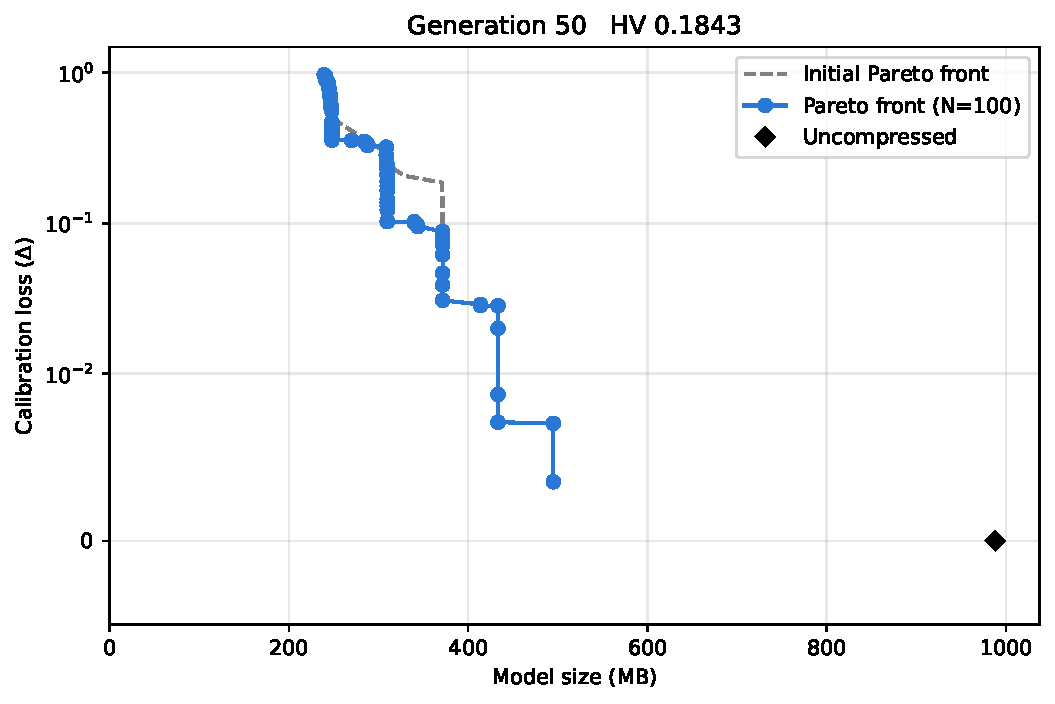
\includegraphics[width=0.75\linewidth]{figures/pareto_front.pdf}
\caption{Final Pareto front (100 solutions) of calibration $\dloss$ against encoded size, with the
front of the initial population and the uncompressed model.}
\label{fig:front}
\end{figure}

\begin{figure}[!p]
\centering
\begin{subfigure}{0.8\linewidth}
  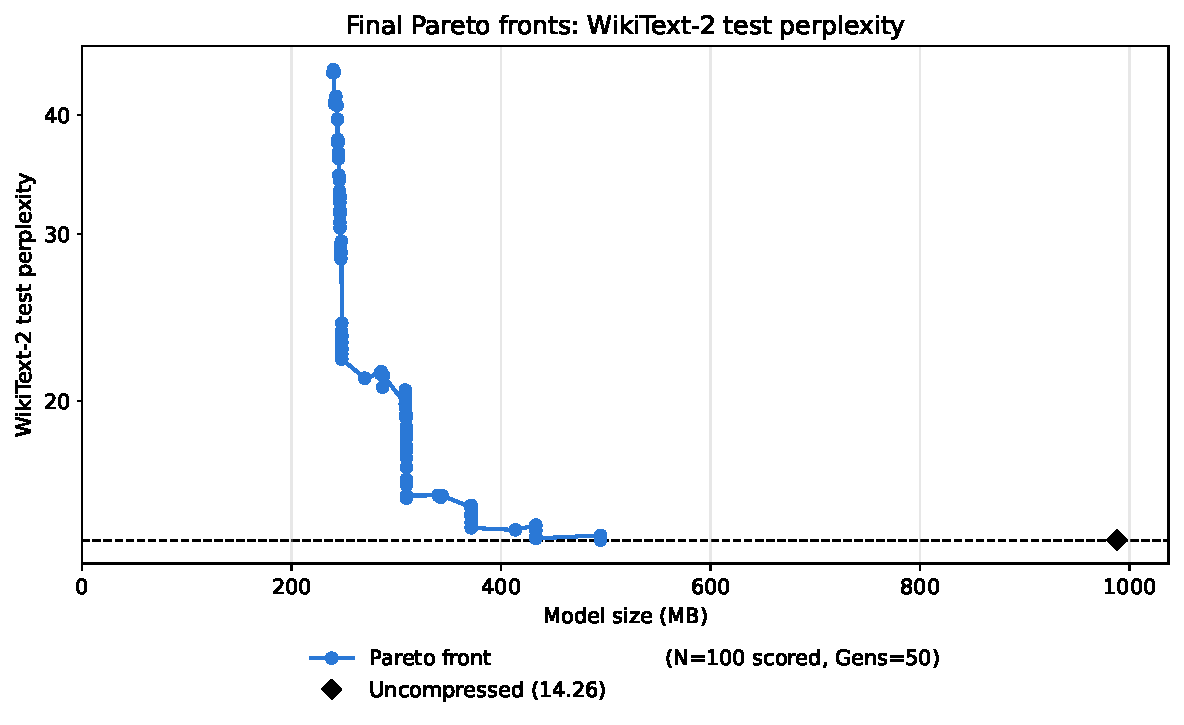
\includegraphics[width=\linewidth]{figures/test_front_wikitext2.pdf}
  \caption{WikiText-2 test}
\end{subfigure}\\[8pt]
\begin{subfigure}{0.8\linewidth}
  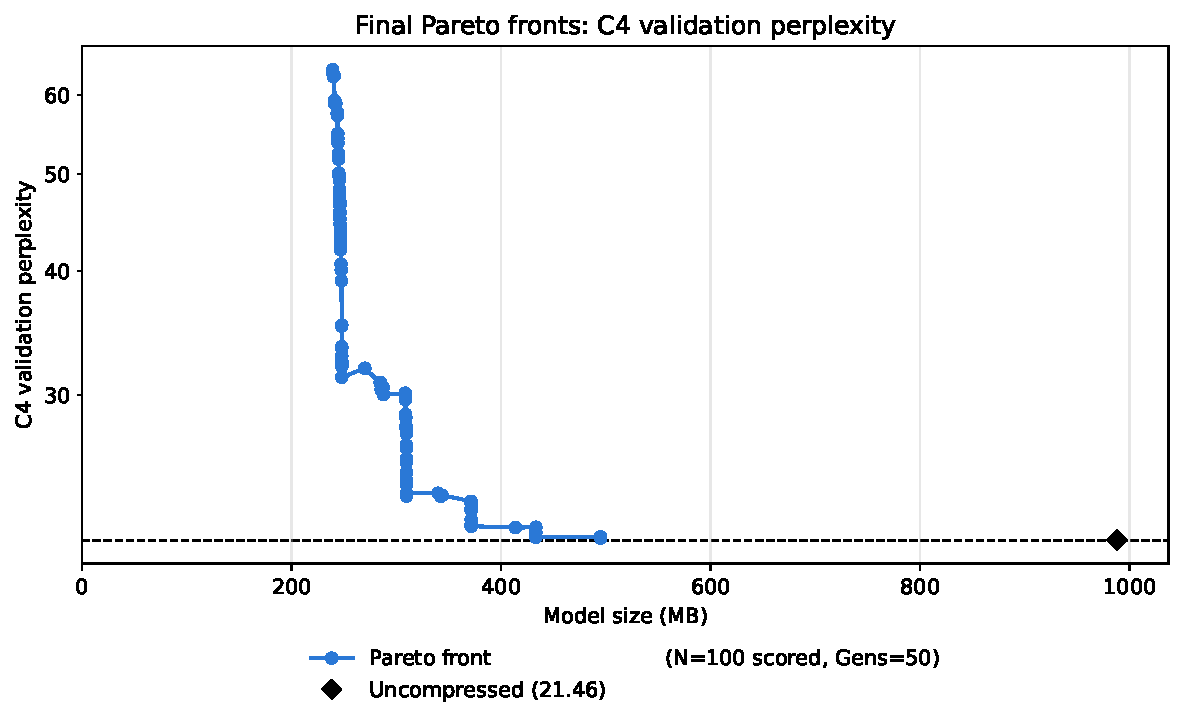
\includegraphics[width=\linewidth]{figures/test_front_c4.pdf}
  \caption{C4 validation}
\end{subfigure}
\caption{Test perplexity of the final Pareto front against encoded size. The dashed line is the
uncompressed model.}
\label{fig:testfront}
\end{figure}

\section{Selected models}

The calibration error of a solution is $\dloss/\mathcal{L}_0$. For each level (0, 1, 2, 5, 10\%) the
smallest solution within it is selected. No solution has zero error, so the most accurate one (0.12\%)
stands for the 0\% level. Every solution smaller than 309\,MB exceeds 10\% error, so the
5\% and 10\% models are nearly the same size but reach it with different settings: Q10 prunes more
($\beta=0.32$ against $0.02$) and clips harder ($c=0.85$ against $0.93$).

\begin{table}[htbp]
\centering
\footnotesize
\setlength{\tabcolsep}{3.5pt}
\begin{tabular}{lrrrrrrrrrr}
\toprule
Model & $k$ & $c$ & Sparsity & Calib. err. & Size & Smaller & Bits/w & Huffman & WikiText-2 & C4 \\
      &     &     & (\%)     & (\%)        & (MB) & by      &        & bits/w  & ppl        & ppl \\
\midrule
Uncompressed (bf16) & --  & --    & 0.0  & 0.00 & 988 & 1.00$\times$ & 16.00 & --   & 14.26 & 21.46 \\
\addlinespace
Q0  (0\%)  & 164 & 0.995 & 2.2  & 0.12 & 495 & 2.00$\times$ & 8.02 & 6.47 & 14.26 & 21.55 \\
Q1  (1\%)  & 65  & 0.934 & 5.3  & 1.00 & 414 & 2.39$\times$ & 6.70 & 5.23 & 14.61 & 22.08 \\
Q2  (2\%)  & 52  & 0.949 & 6.8  & 1.61 & 372 & 2.66$\times$ & 6.01 & 4.84 & 15.08 & 22.49 \\
Q5  (5\%)  & 29  & 0.928 & 11.8 & 4.75 & 310 & 3.19$\times$ & 5.01 & 4.05 & 17.00 & 25.05 \\
Q10 (10\%) & 28  & 0.849 & 19.2 & 9.87 & 309 & 3.20$\times$ & 5.00 & 3.98 & 20.52 & 29.70 \\
\bottomrule
\end{tabular}
\caption{Selected solutions. Sparsity counts pruned weights and weights rounded to zero. Huffman bits/w
is the storage with Huffman-coded codes (reported only, not optimized). None of the five merges levels
($\rho=1$).}
\label{tab:models}
\end{table}

\section{Benchmark protocol}

All models are evaluated with the same harness (lm-evaluation-harness 0.4.13), in bf16, on full
evaluation splits, without a chat template, with fixed seeds. Compressed weights are reconstructed in
place, so the models differ only in their weight values.

\begin{table}[htbp]
\centering
\small
\begin{tabular}{llrcl}
\toprule
Benchmark & Split & Questions & Shots & Metric \\
\midrule
PIQA          & validation & 1{,}838  & 0 & accuracy, length-normalized \\
ARC-Easy      & test       & 2{,}376  & 0 & accuracy, length-normalized \\
ARC-Challenge & test       & 1{,}172  & 0 & accuracy, length-normalized \\
HellaSwag     & validation & 10{,}042 & 0 & accuracy, length-normalized \\
WinoGrande    & validation & 1{,}267  & 0 & accuracy \\
BoolQ         & validation & 3{,}270  & 0 & accuracy \\
MMLU          & test       & 14{,}042 & 5 & accuracy (57 subjects) \\
GSM8K         & test       & 1{,}319  & 5 & exact match of the final number \\
\bottomrule
\end{tabular}
\caption{Benchmarks. Multiple-choice tasks pick the answer with the highest log-likelihood; GSM8K
generates a solution and compares the extracted final number with the reference.}
\label{tab:protocol}
\end{table}

\clearpage
\section{Results}

\begin{table}[!ht]
\centering
\small
\setlength{\tabcolsep}{4pt}
\begin{tabular}{lrrrrrrrrrr}
\toprule
Model & Size & PIQA & ARC-e & ARC-c & HellaS. & WinoG. & BoolQ & MMLU & GSM8K & Average \\
      & (MB) &      &       &       &         &        &       & 5-shot & 5-shot &       \\
\midrule
Uncompressed & 988 & 70.4 & 59.2 & 33.1 & 52.4 & 56.0 & 67.8 & 47.0 & 31.2 & 52.1 \\
\addlinespace
Q0  (0\%)    & 495 & 70.2 & 59.9 & 33.5 & 52.4 & 56.6 & 68.4 & 47.0 & 31.7 & 52.5 \\
Q1  (1\%)    & 414 & 70.2 & 59.6 & 33.7 & 52.5 & 55.9 & 64.3 & 46.5 & 27.6 & 51.3 \\
Q2  (2\%)    & 372 & 69.5 & 61.0 & 32.8 & 52.0 & 54.2 & 66.6 & 46.1 & 26.7 & 51.1 \\
Q5  (5\%)    & 310 & 69.2 & 55.2 & 32.0 & 50.0 & 56.4 & 49.7 & 45.0 &  9.7 & 45.9 \\
Q10 (10\%)   & 309 & 67.5 & 56.2 & 31.0 & 47.7 & 57.2 & 56.1 & 38.3 & 12.6 & 45.8 \\
\midrule
Std. error   &     & 1.1  & 1.0  & 1.4  & 0.5  & 1.4  & 0.8  & 0.4  & 1.3  &      \\
\bottomrule
\end{tabular}
\caption{Accuracy (\%, higher is better), with the unweighted average over the eight benchmarks. Last
row: standard error of the uncompressed model's accuracy.}
\label{tab:results}
\end{table}

\begin{table}[!ht]
\centering
\small
\setlength{\tabcolsep}{4pt}
\begin{tabular}{lrrrrrrrrrr}
\toprule
Model & Size & PIQA & ARC-e & ARC-c & HellaS. & WinoG. & BoolQ & MMLU & GSM8K & Avg.\ kept \\
      & (MB) &      &       &       &         &        &       &      &       & (\%)       \\
\midrule
Q0  (0\%)  & 495 & $-0.2$ & $+0.7$ & $+0.4$ & $-0.1$ & $+0.6$ & $+0.6$  & $\phantom{+}0.0$ & $+0.5$ & 100.6 \\
Q1  (1\%)  & 414 & $-0.2$ & $+0.5$ & $+0.6$ & $\phantom{+}0.0$ & $-0.2$ & $-3.5$ & $-0.4$ & $-3.6$ & 98.4 \\
Q2  (2\%)  & 372 & $-0.9$ & $+1.9$ & $-0.3$ & $-0.5$ & $-1.8$ & $-1.2$  & $-0.8$ & $-4.5$  & 98.0 \\
Q5  (5\%)  & 310 & $-1.2$ & $-4.0$ & $-1.1$ & $-2.4$ & $+0.3$ & $-18.1$ & $-2.0$ & $-21.5$ & 88.0 \\
Q10 (10\%) & 309 & $-2.9$ & $-2.9$ & $-2.1$ & $-4.7$ & $+1.2$ & $-11.8$ & $-8.6$ & $-18.6$ & 87.9 \\
\bottomrule
\end{tabular}
\caption{Change in accuracy against the uncompressed model (percentage points; negative is a loss).
Avg.\ kept is the compressed model's average accuracy as a percentage of the uncompressed model's.}
\label{tab:delta}
\end{table}

\FloatBarrier
\paragraph{Observations.}
\begin{itemize}
  \item \textbf{8 bits per weight is lossless.} Q0 is $2.00\times$ smaller and every benchmark is
        within 0.7 points of the uncompressed model, inside the standard errors (100.6\% kept).
  \item \textbf{1--2\% calibration error keeps 98\% of the accuracy.} Q1 and Q2 are $2.39\times$ and
        $2.66\times$ smaller. The commonsense tasks and MMLU stay within 2 points; GSM8K drops 3.6--4.5
        points and BoolQ up to 3.5.
  \item \textbf{At 5.0 bits per weight, about 12\% of the average accuracy is lost.} Q5 and Q10 are
        $3.2\times$ smaller and keep 88\%. The commonsense tasks lose at most 5 points; BoolQ breaks
        (Q5: 49.7\%, below the 62.2\% of always answering ``yes'').
  \item \textbf{GSM8K is the most sensitive benchmark:} 31.2\% uncompressed, 27--28\% at 1--2\%
        error, 10--13\% at 5--10\% error.
  \item \textbf{Calibration loss does not rank the models downstream.} Q5 has half the calibration
        error of Q10 and lower test perplexity, and is better on MMLU (45.0 against 38.3), but worse on
        BoolQ and GSM8K; the two averages are equal. Below about 6 bits per weight, models need a
        benchmark check before use.
\end{itemize}

\end{document}
